\section{Challenges}

What challenges have occurred for this week?

A challenge we had with the implementing the pathfinding scene into the main Unity scene was configuring the correct places that the agent is allowed to traverse. 

\begin{figure}[htb]
    \centering
    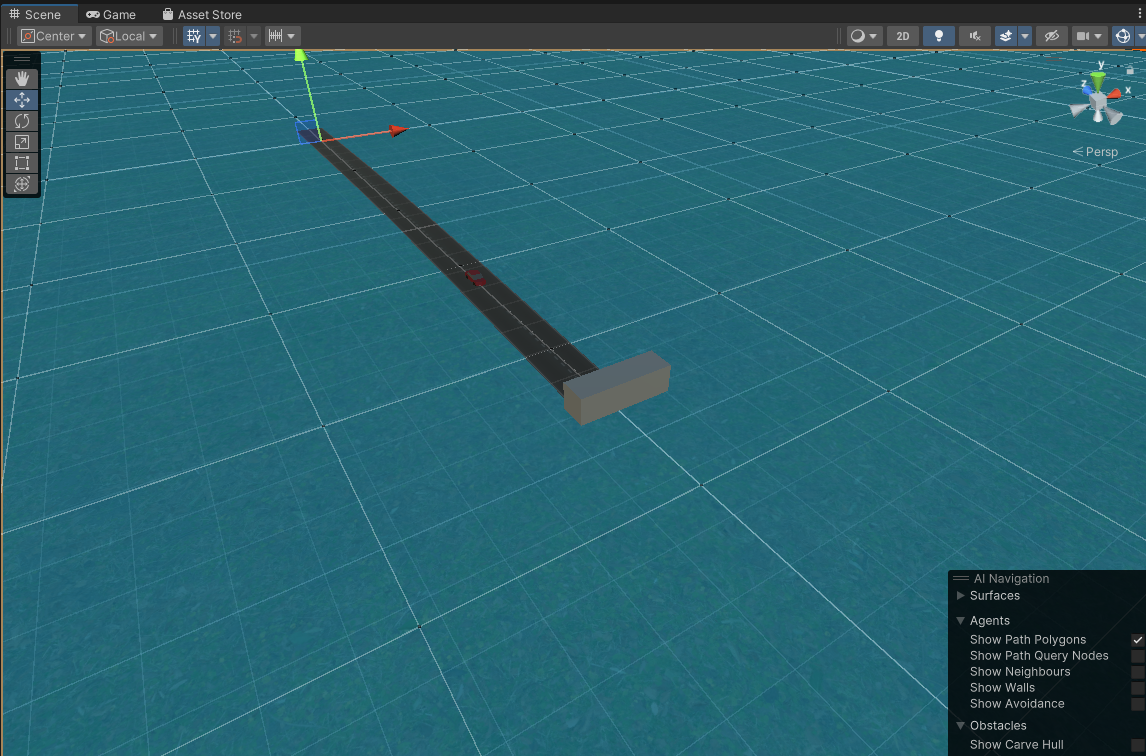
\includegraphics[width=10cm]{../Images/Update3/WrongMesh.png}
       \caption{The baked Nav Mesh recognizing everything but the road we want the car to go on.}
           \label{Fig:Wrong Path}
\end{figure}

\begin{flushleft}
The blue represents the path that the program will let the car traverse. This is a problem because the mesh covers every part of the plain but the actual road that we want the car to stick to. Fortunately, this isn't a very hard fix but just took a good amount of research. We just need to make sure the "Navigation Static" option below was ticked off.
\end{flushleft}

\begin{figure}[!ht]
    \centering
    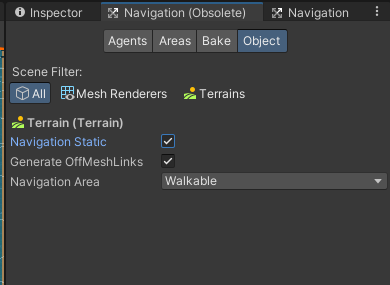
\includegraphics[width=10cm]{../Images/Update3/MeshSetting.png}
       \caption{The settings we need to keep an eye out for.}
           \label{Fig: Bake Mesh Settings}
   \end{figure}

\begin{figure}[!ht]
    \centering
    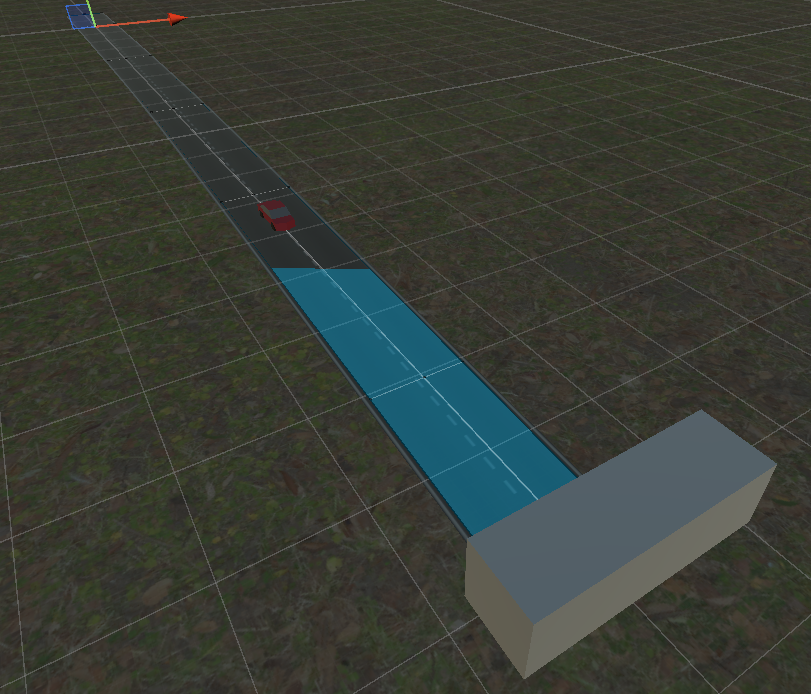
\includegraphics[width=10cm]{../Images/Update3/CorrectMesh.png}
       \caption{Though it's hard to see in the screenshot, as you go through the scene the whole road is blue and it's correctly baked.}
           \label{Fig: Bake Mesh Settings}
\end{figure}

\begin{flushleft}
Additionally, there's currently a problem that the model for the Sedan is by default upright, so we'd need to change the model somehow. 
\end{flushleft}

Obtaining the information to use for the TomTom API was rather interesting.
The documentation was clear, but very segmented; The information was spread across several pages that were not all accessible from each other.
A difficult challenge was deciding which API's to utilize (since this meant we might have to change the access key).
We are considering utilizing multiple API's and combining the images together to get a more complete sense of direction/understanding of the area.